\documentclass[12pt]{article}
% Packages and macros
\usepackage[T1]{fontenc}
\usepackage{mathptmx}
\usepackage{pgf}
\usepackage{pgfpages}
\usepackage{parallel}
\usepackage{siunitx}
\usepackage{booktabs}
\usepackage{fancyhdr}
\usepackage{datetime}
%\usepackage[utf8]{inputenc}
\usepackage{graphicx}
\usepackage{blindtext}
\usepackage{multicol}
\usepackage{enumerate}
\usepackage{pifont}
\usepackage{amssymb}
\usepackage[export]{adjustbox}
\usepackage[margin=1in]{geometry}
\usepackage[francais]{babel}
\usepackage{caption}
\newcommand{\source}[1]{\vspace{-12pt} \caption*{Source: {#1}} }
\usepackage{amsmath}
\usepackage{xcolor}
\usepackage{array}
\usepackage{tabularx}
\usepackage[thinlines]{easytable}

\newdateformat{monthyeardate}{%
  \monthname[\THEMONTH], \THEYEAR}

\pgfpagesdeclarelayout{boxed}
{
  \edef\pgfpageoptionborder{0pt}
}
{
  \pgfpagesphysicalpageoptions
  {%
    logical pages=1,%
  }
  \pgfpageslogicalpageoptions{1}
  {
    border code=\pgfsetlinewidth{1pt}\pgfstroke,%
    border shrink=\pgfpageoptionborder,%
    resized width=.98\pgfphysicalwidth,%
    resized height=.98\pgfphysicalheight,%
    center=\pgfpoint{.5\pgfphysicalwidth}{.5\pgfphysicalheight}%
  }%
}
\pgfpagesuselayout{boxed}
\setlength{\columnsep}{0.5cm}

% \renewcommand\thesubsection{\Alph{subsection}}

\begin{document}
\pagestyle{fancy}
\lhead{MINF}
\chead {\today}
\rhead{TP2}
\fontsize{16}{16}\selectfont

% ------------------------- TITLE PAGE INSERTION ------------------------ 
\begin{titlepage}
   \begin{center}
        \vspace*{1cm}
        \LARGE
        \textbf{Microinformatique \\ Travail pratique 2}
        
        \vspace{0.3cm}
       	Mise en place d'une communication USART sur PIC32
            
        \vspace{1.5cm}

        \textbf{Meven Ricchieri \\ Ali Zoubir}

        \vfill
            
        Rapport de  laboratoire
            
        \vspace{0.8cm}
     
        
\includegraphics[width=0.31\textwidth]{./ETML-ES-LOGO.png}

        Génie électrique\\
        École supérieure\\
        Suisse\\
        \monthyeardate\today
            
   \end{center}
\end{titlepage}
\clearpage


% --------------------- TABLE OF CONTENTS  ------------------------------- 
\tableofcontents
\clearpage

% ------------------------- INTRODUCTION --------------------------------- 
\section{Introduction}
L'objectif de ce deuxième travail pratique est de permettre le réglage de la vitesse et de l'angle du moteur et du servomoteur par communication RS232, en utilisant la même application sur deux kits qui communiqueront entre eux par un câble croisé ou plus tard, un kit et une application C\# sur un PC.

\clearpage


% ------------------- PRELIMINARY TASK (TASK0) --------------------------- 
% ------------------------- INTRODUCTION --------------------------------- 
\section{Introduction}
L'objectif de ce travail pratique est de mettre en place une communication USART sur un PIC32.

Pour se faire, nous allons graphiquement initialiser le périphérique série, puis programmer selon le CDC ainsi que les différents supports de cours afin de permettre une communication entre différent KIT MCU.


% ------------------------- PRELIMINARY TASK -----------------------------
\section{Initialisation graphique USART}
{
    Nous avons configuré graphiquement par Harmony un périphérique USART avec les caractéristiques suivantes :
    
    \fbox{57600 Baud} \fbox{Priorité int. niveau 5} \fbox{Static} \vspace{+4mm}
    
    Nous avons ensuite dû modifier la routine d'interruption ainsi que différentes fonctions des librairies fournies dans le cadre de ce TP.    
}

\clearpage
\section{Mesures}
{
	\subsection{Liste de matériel}
	{
		\begin{flushleft}
			\underline{Liste de matériel :}\\
			Oscilloscope \textbf{P1} \ : \qquad ES.SLO2.05.01.12\\
			Alimentation \textbf{G1} \ : \qquad ES.SLO2.00.00.24\\
			Kit de développement : ES.SLO2.00.05.36
		\end{flushleft}
	
		\begin{figure}[h]
			\centering
			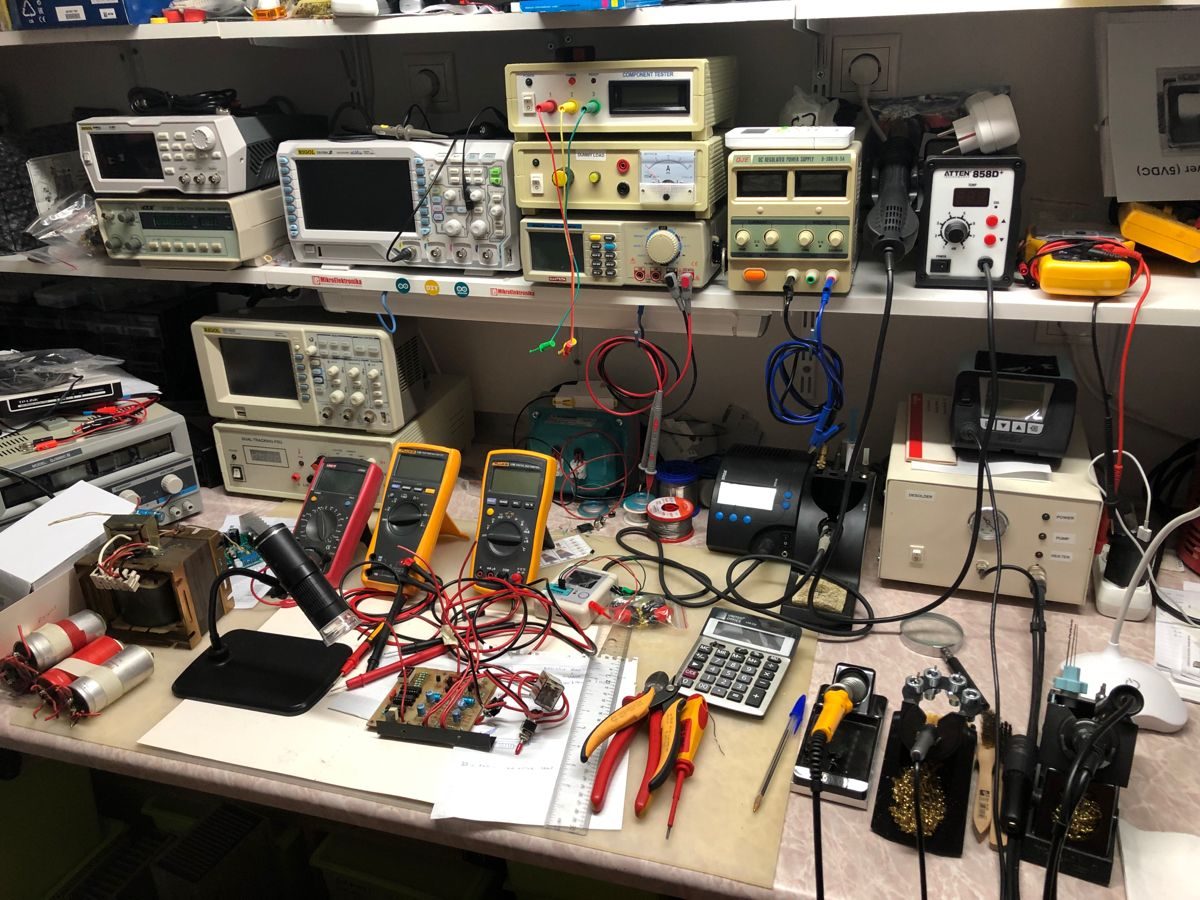
\includegraphics[width=0.7\linewidth]{IllustrationLab}
			\caption{Illustration}
			\label{fig:illustrationlab}
			\source{https://www.pinterest.com/pin/electronics-lab--819092250979124500/}
		\end{figure}
		
	}
	\clearpage
	\subsection{Schéma de mesure}
	{
		\subsubsection{Mesure des diodes, comportements des interruption}
		\begin{figure}[h]
			\centering
			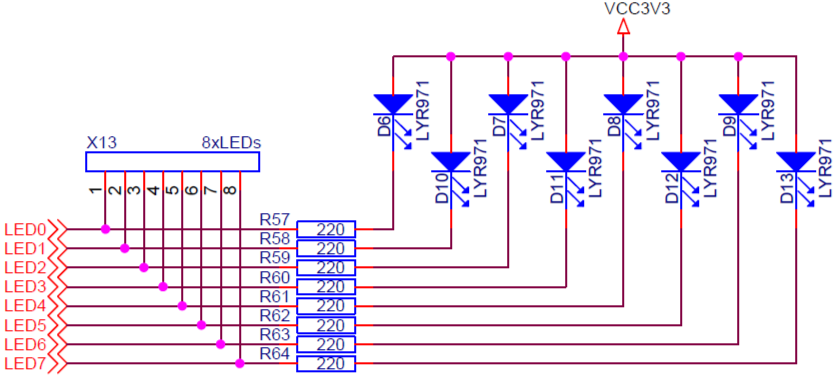
\includegraphics[width=0.55\linewidth]{SchemaDiode}
			\caption{Schéma mesure des diodes}
			\label{fig:schemadiode}
		\end{figure}
	
	\subsubsection{Mesure des trames Tx Rx}
	\begin{figure}[h]
		\centering
		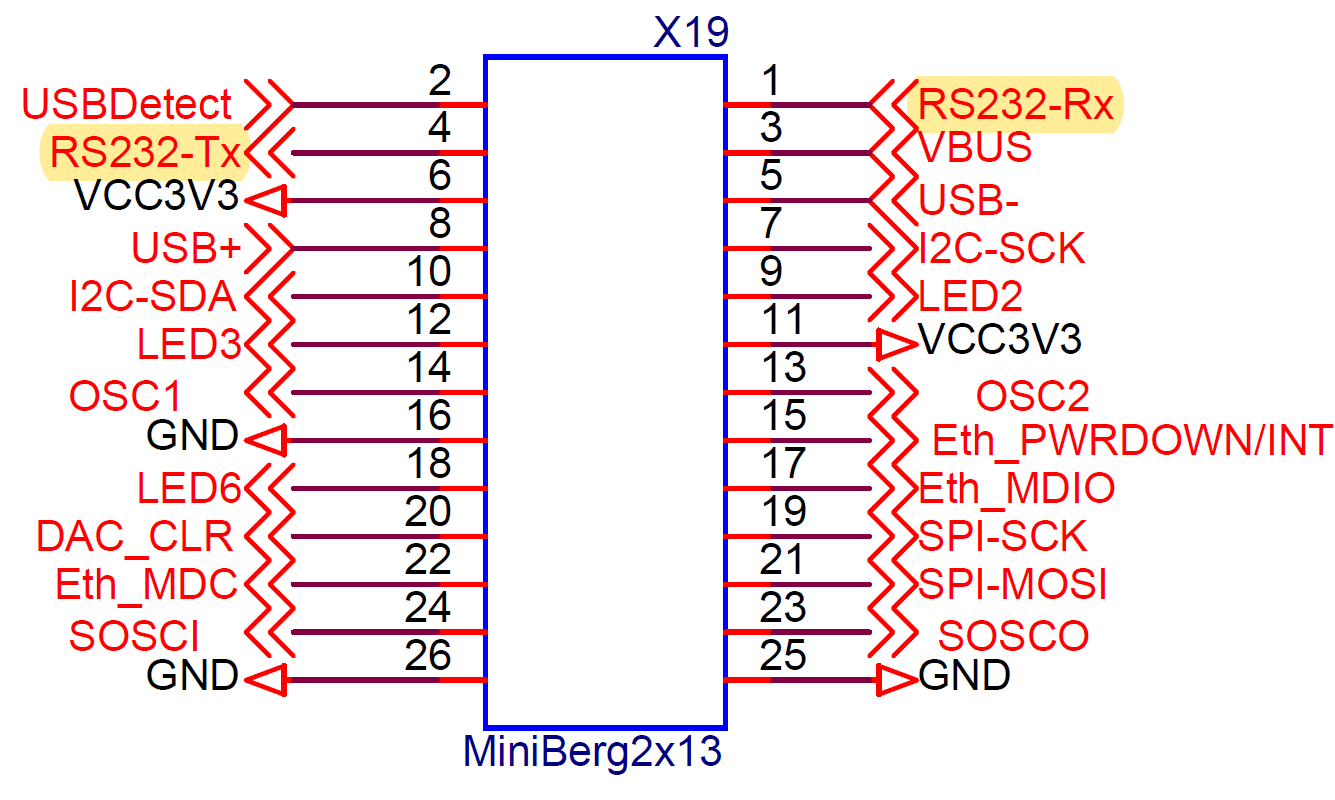
\includegraphics[width=0.45\linewidth]{SchemaRxTx}
		\caption{Schéma de mesure des trames USART}
		\label{fig:schemarxtx}
	\end{figure}
		\begin{table}[!h]
	\centering
	\begin{tabular}{c|c|c|c}
		Sonde & Connecteur & Label & Label secondaire \\
		\hline\hline
		CH1 & X19-4 & RS232-Tx & ConRS232-Rx \\
		CH2 & X19-1 & RS232-Rx & ConRS232-Tx \\
		CH3 & X13-4 & D11 & LED3 \\
		CH4 & X13-5 & D8 & LED4 \\
		CH2' & X13-6 & D12 & LED5 \\
	\end{tabular}
		\caption{Emplacements des sondes de mesures}
		\label{tab:tableauSondes2}
	\end{table}
	}
	
	\clearpage
	\subsection{Mesures et commentaires}
	{
		\subsubsection{Mesure}
		
		Ici nous mesurons la trame Rx du PIC, ainsi que les diode indiquant l'état des différentes interruptions.
		
		\centering
		\fbox{LED3 : Durée interruption} \fbox{LED4 : interruption réception}
		
		\begin{figure}[h]
			\centering
			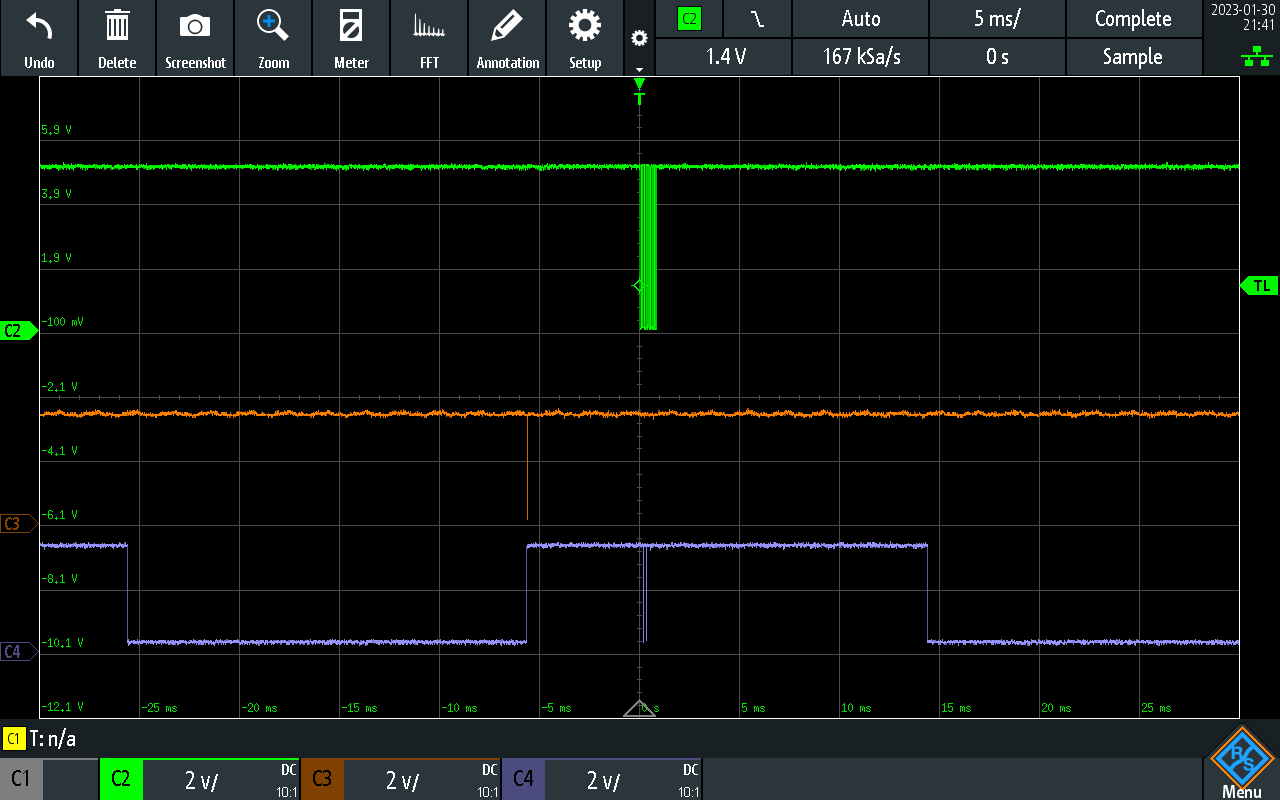
\includegraphics[width=0.55\linewidth]{MesuresLedsRx}
			\caption{Mesure Rx et diodes}
			\label{fig:mesuresledsrx}
		\end{figure}
		Nous pouvons constater que l'interruption USART à lieu avant les données reçues et déclenche directement le traitement Rx dans l'interruption.
		
		\begin{figure}[h!]
			\centering
			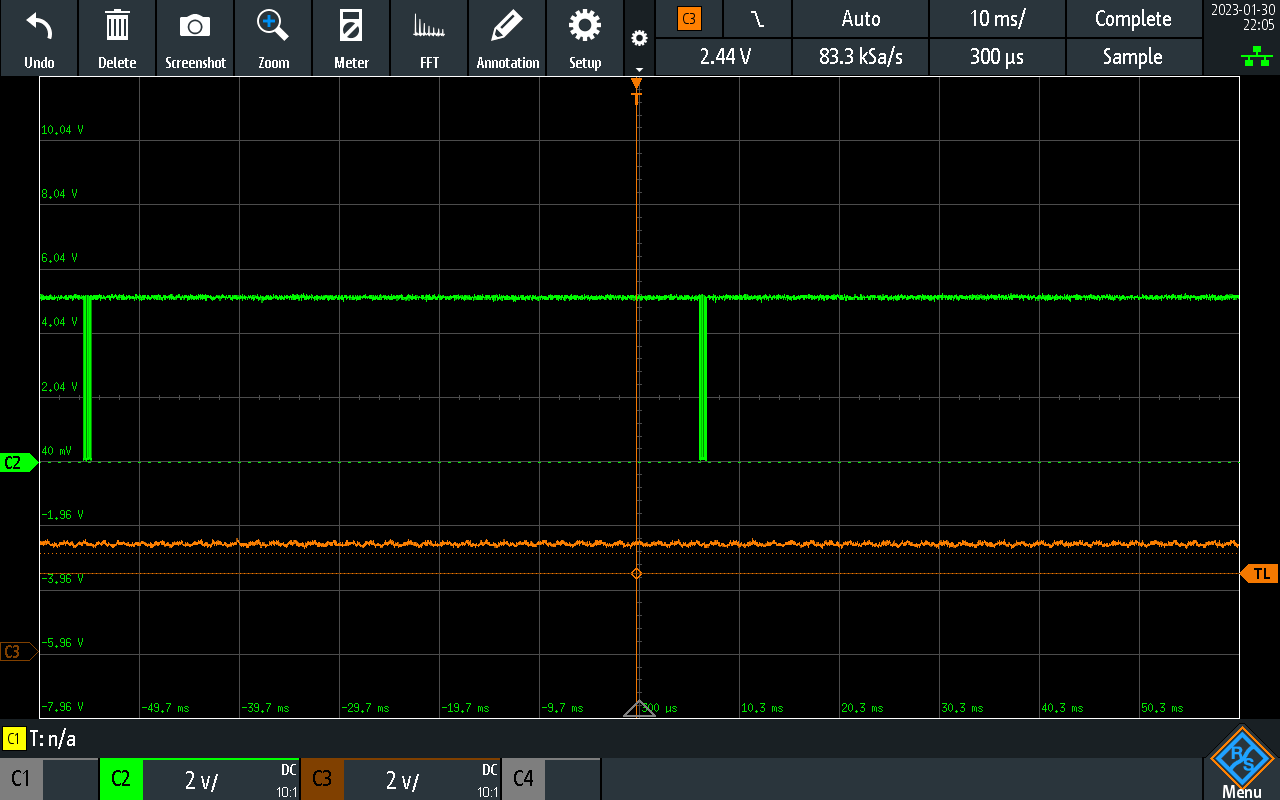
\includegraphics[width=0.55\linewidth]{MesureRxErrCRC}
			\caption{Mesure trame Rx et erreur CRC}
			\label{fig:mesurerxerrcrc}
		\end{figure}
		Nous n'obtenons pas d'erreurs de CRC, car le logiciel lors de l'envoi d'un CRC tronqué, n'envoie que 3 bytes concrets, hors l'algorithme filtre l'erreur directement au start avant le contrôle CRC. Si une trame concrète de 5 bytes est envoyée avec un mauvais CRC, l'erreur est détectée.
		
	}    
}

\clearpage
\section{Conclusion}
{
	Nous avons pu mettre en place une communication série entre deux kit PIC32 ETML-ES dont un simulé par un logiciel POO sur l'ordinateur. 
	
	Nous nous sommes sensibilisés aux fonctionnement d'un périphérique USART et de ces différents registres ainsi que de l'utilisation d'un FIFO software dont nous venons traiter les données pour la réception ainsi que l'émission. 
	
	\vspace{125mm}
	\begin{tabular}{@{}p{2.5in}p{2in}p{2in}@{}}
		Lausanne, \today\\
		ETML-ES \vspace{+20mm}\\
		\hrulefill && \hrulefill\\
		Meven Ricchieri && Ali Zoubir\\
	\end{tabular}
}

% ------------------------ MAIN TASK (TASK1) ----------------------------- 
% ------------------------- MAIN TASK ---------------------------------
\section{Main task}

\clearpage

\end{document}
